%=====================================================
%====== If you are new to LaTeX, this website ========
%======     will be your new best friend:     ========
%======   http://en.wikibooks.org/wiki/LaTeX  ========
%======   Template created by Jonathan Blair  ========
%=====================================================



%=====================================================
%============ Controls ===============================
%=====================================================

%\documentclass[12pt,letterpaper,onecolumn]{article}
\documentclass[11pt,letterpaper,onecolumn]{article}
%\documentclass[10pt,letterpaper,onecolumn]{article}  % not recommended
%\documentclass[12pt,letterpaper,twocolumn]{article}
%\documentclass[11pt,letterpaper,twocolumn]{article}
%\documentclass[10pt,letterpaper,twocolumn]{article}


\usepackage{amsmath}
\usepackage{graphicx}
\usepackage{url}
\usepackage{textgreek}
\usepackage{float}
\usepackage{booktabs}
\usepackage{subcaption}
%\graphicspath{{path-to-folder-containing-necessary-graphics}{other folder as necessary}}


%=====================================================
%============ \begin{document} =======================
%=====================================================

\begin{document}

%=====================================================
%============ Title ==================================
%=====================================================

\title{\bf Observation of the Behavior of an Operational Amplifier in a Differentiation, Integration and Comparator Circuit}
%\title{\Large\bf Larger, Bolded Title}

%=====================================================
%============ Author =================================
%=====================================================
\author{
 Jairo Portillo \\*
  \\*
 PHY 338K Electronic Techniques \\*
 Department of Physics \\*
 The University of Texas at Austin \\*
 Austin, TX 78712, USA
}
\date{May 6, 2016}

%\address{The University of Texas, Austin, Texas, 78712}

\maketitle

%=====================================================
%============ Abstract ===============================
%=====================================================

\begin{abstract}

In this lab, we will explore the behavior of a Operational Amplifier as it influences differentiation and integration of the input signal. We also observed the behavior of comparator circuits and verify hysteresis along with its immunity to noise.

\end{abstract}

%=====================================================
%============ Body of the article ==========================
%=====================================================

%=====================================================
%============ Section ==================================
%=====================================================

\section{Preperation}

 In order to prepare for this lab, we must review the behavior of Operational amplifiers and differentiation and integrator circuits. If we recall for the RC circuits lab we know that for a differentiating circuits that the output voltage is
$$V_{out} \approx RC\frac{d}{dt}V_{in}$$
and for integrator circuits that the output voltage is
$$V_{out} \approx \frac{1}{RC}\int^t_0 V_{in}\,dt$$
We know that an op-amp has two inputs an inverting and not inverting.Since we are using the inverting input we know that $V_{in} \Rightarrow -V_{out}$ or $-V_{in} \Rightarrow V_{out}$. Thus we see that for the Op amp circuits we expect
$$V_{out} \approx -RC\frac{d}{dt}V_{in}$$
and
$$V_{out} \approx -\frac{1}{RC}\int^t_0 V_{in}\,dt$$

\begin{figure}[H]
\begin{subfigure}{.5\textwidth}
  \centering
  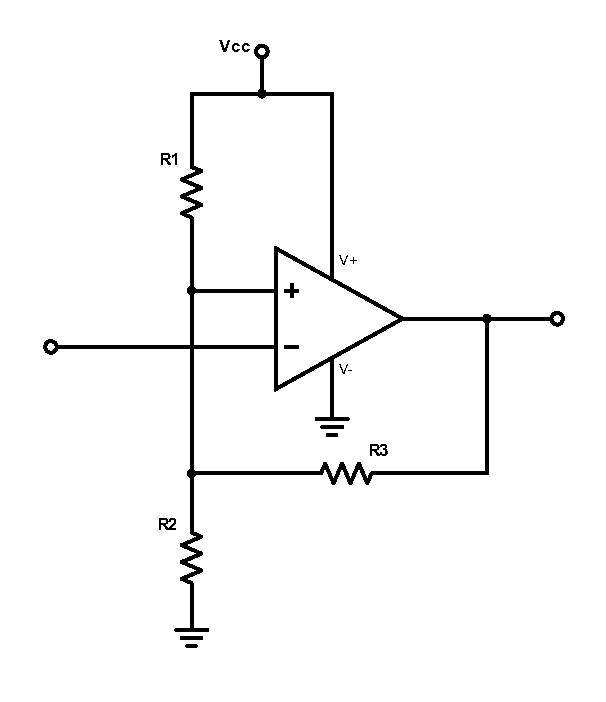
\includegraphics[scale =.6]{Lab-10-w-feedback.pdf}
  \caption{With Feedback}
  \label{fig:sub1}
\end{subfigure}%
\begin{subfigure}{.5\textwidth}
  \centering
  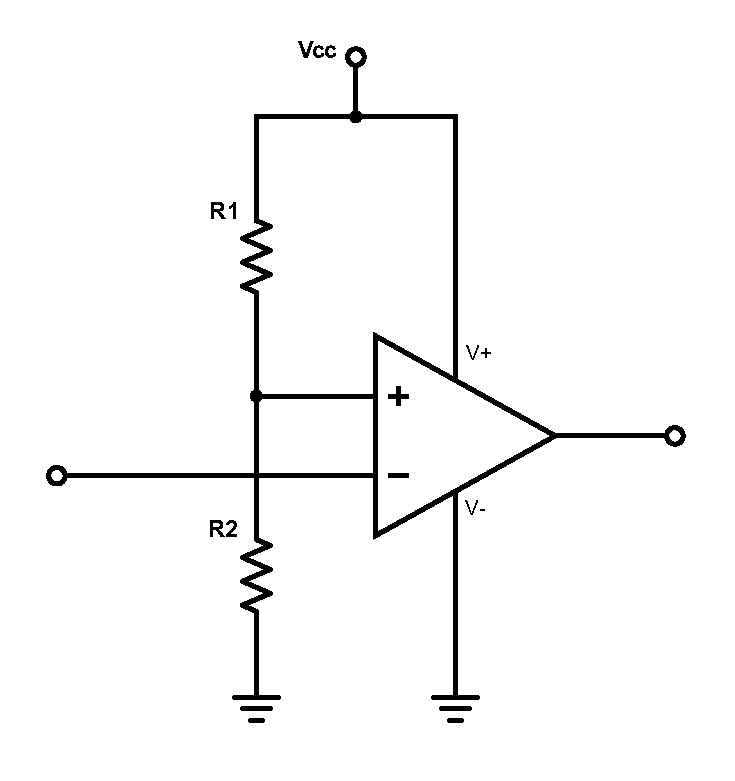
\includegraphics[scale=.5]{Lab-10-wo-feedback.pdf}
  \caption{Without Feedback}
  \label{fig:sub2}
\end{subfigure}
\caption{Voltage Comparators}
\label{fig:test}
\end{figure}

The voltage comparator circuit simply compares to inputs and determines which one is greater. The output switched from positive to negative depending on which of the inputs is greater. The threshold at which the output switches can be observed. This threshold voltage can be found by
$$V_T=\frac{R_2}{R_1 + R_2}V_{cc}$$
where $V_{cc}$ is the voltage from the DC supply. The disadvantage this circuit has are that for slow varying inputs, the output swing can be slow and that is if the input is noisy, the output may take several transitions as the input passes the threshold voltage. Positive feedback solves this issue as the resistor $R_3$ causes the circuit to have two thresholds depending on the output. This causes hysteresis as the output depends on the input voltage and on its recent output. This new threshold is known as the Schmitt Trigger and yields a ratio of 
$$ \lambda = \frac{R_2}{R_2 + R_3}$$
With this ratio we can find the new threshold voltage
$$V_T = \frac{R_2}{R_2 + R_3}V_{cc}$$
and the hysteresis voltage can be found
$$V_H = V_{T}^{+} - V_{T}^{-} = 2\lambda V_{cc}$$

\section{Lab work}

\subsection{Apparatus}


This lab will use a signal generator, an oscilloscope, two DC voltage sources, an op-amp, a .39 $\mu$F capacitor, a 25 pf, a 10k$\Omega$ resistors, 102.7k$\Omega$ resistor and a 100k$\Omega$ resistor. The AC signal generator will be directly connected to the inverting input of the op amp. A Tee connector will connect the input AC signal with channel 1 on the oscilloscope. The output will be connected to Channel 2. For Configurations of the resistors refer to Fig 1 and Fig 2 below where $R_1 = 10k\Omega$, $R_2 = 102.7k\Omega$, and $R_3 = 100k\Omega$.

\begin{figure}[H]
    \centering
    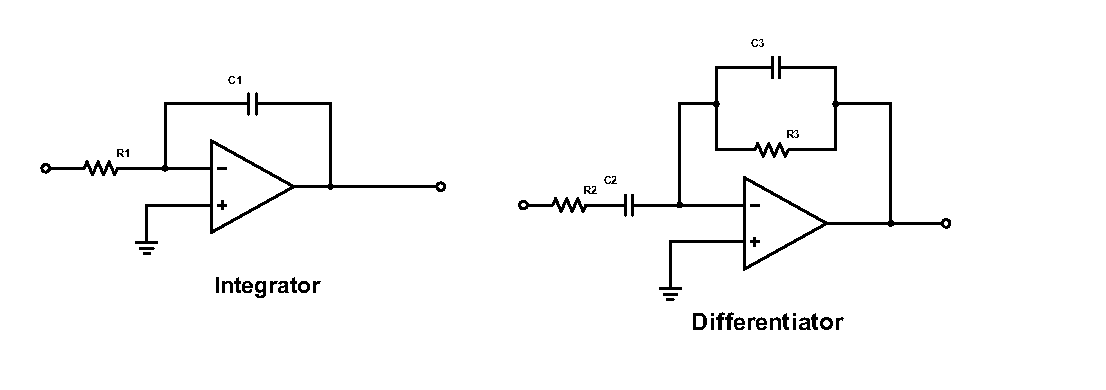
\includegraphics[scale = .8]{lab10IntDif.pdf}
    \caption{The Integrator and Differentiator Circuits}
    \label{fig:my_label}
\end{figure} 

For the integrator and differentiator circuits $R_1 = R_2 = 10k\Omega$, $ R_3 = 102.7k\Omega$, $C_2 = .1\mu F$,and $C_3 = 25pf$.

\subsection{Data Collection}

For the integrator, we found the corner frequency to be 243.9 Hz from the oscilloscope while the calculated frequency was 256.41 Hz. The triangle was was integrated to a sine wave as expected and as observed from the low pass filter. However, in this case we see that $V_{out} \ll V_{in}$ is no longer true due to the op amp.For the differentiator, we observed that a triangle wave input had a square wave output. The two corner frequencies found were 425.8 Hz and 2.825 kHz, while the expected values were found to be 1kHz and 4kHz. 

For the voltage comparator, we found the threshold voltage to be 14.6V and calculated it to be $\frac{102.7k\Omega}{112.7k\Omega}15V=13.6V$. The comparator circuit with feedback had a threshold voltage of 7.3v which is 1\% from the calculated value of 7.24V.

\section{Summary and conclusions}

In this lab, we have seen how an operational amplifier influences the out put of integrating and differentiating circuits. It maintains the expected function but does not inhibit any output. We found the corner frequencies to be 243.9 Hz for the integrator and 425.8 Hz and 2.825 kHz for the differentiator. We also observed how a feedback comparator was resistant to any input noise and it had a threshold of 7.3V. 



%=====================================================
%============ Bibliography  ==============================
%=====================================================



%=====================================================
%============ End ====================================
%=====================================================

\end{document}

%=====================================================
%============ End ====================================
%=====================================================